\section{正交基}
\label{sec:ipspace-orthonormal-bases}

有限维内积空间中，标准正交基让坐标的计算变得简单：第$j$个坐标就是与第$j$个基向量的内积。无限维中，第~\ref{chap:functions-as-vectors}章已经看到代数基只允许有限组合，常常无法写出，也不适合谈论级数。本节换一种要求：不要求每个元素都是有限个方向的组合，只要求它能被这些方向的有限组合以任意精度逼近。

\paragraph{标准正交系}
先给出两两正交、长度为$1$的一族元素。

\begin{definition}[标准正交系]
\label{def:ipspace-orthonormal-system}
内积空间$H$中的一族元素$\{e_i\}_{i\in I}$称为\term{标准正交系}（orthonormal system），若对所有$i,j\in I$，
\[
 \langle e_i,e_j\rangle=\delta_{i,j}=\begin{cases}1,&i=j,\\0,&i\neq j.\end{cases}
\]
\end{definition}

标准正交系总是线性无关的：若$\sum_{k=1}^nc_ke_{i_k}=0$，与$e_{i_j}$作内积得$c_j=0$。$\ell^2$中的标准单位列$\{e_k\}_{k\geq1}$是标准正交系；上一节的$\{e^{\mathrm ikx}/\sqrt{2\pi}\}_{k\in\mathbb Z}$是$L^2[-\pi,\pi]$中的标准正交系。

\paragraph{Gram--Schmidt正交化}
标准正交系可以从任意线性无关的序列造出来。设$u_1,u_2,\ldots$线性无关，依次令
\[
 v_k=u_k-\sum_{j<k}\langle e_j,u_k\rangle e_j,\qquad e_k=\frac{v_k}{\lVert v_k\rVert}.
\]
$v_k$是$u_k$减去它在$e_1,\ldots,e_{k-1}$方向上的分量，与之前的方向都正交：对$i<k$，$\langle e_i,v_k\rangle=\langle e_i,u_k\rangle-\langle e_i,u_k\rangle=0$。$v_k\neq0$，因为否则$u_k$属于$\operatorname{span}\{e_1,\ldots,e_{k-1}\}=\operatorname{span}\{u_1,\ldots,u_{k-1}\}$，与线性无关矛盾。归纳可知$\operatorname{span}\{e_1,\ldots,e_k\}=\operatorname{span}\{u_1,\ldots,u_k\}$对每个$k$成立。这就是卷二的\term{Gram--Schmidt正交化}（Gram--Schmidt orthogonalization），每一步只涉及有限维子空间，所以可以无限地进行下去。

在$L^2[-1,1]$中对$1,x,x^2,x^3$执行这一过程。$\lVert1\rVert^2=2$，$e_0=1/\sqrt2$。$x$与$1$正交，$\lVert x\rVert^2=\tfrac23$，$e_1=\sqrt{3/2}\,x$。对$x^2$，$\langle e_0,x^2\rangle=\tfrac{\sqrt2}3$，$\langle e_1,x^2\rangle=0$，于是$v_2=x^2-\tfrac13$，这正是上一节向常数投影的误差，$\lVert v_2\rVert^2=\tfrac8{45}$，故
\[
 e_2=\sqrt{\tfrac{45}{8}}\Bigl(x^2-\frac13\Bigr)=\sqrt{\tfrac58}\,(3x^2-1).
\]
对$x^3$，它与偶函数$e_0,e_2$正交，$\langle e_1,x^3\rangle e_1=\tfrac32\cdot\tfrac25x=\tfrac35x$，于是$v_3=x^3-\tfrac35x$，$\lVert v_3\rVert^2=\tfrac27-\tfrac{12}{25}+\tfrac6{25}=\tfrac8{175}$，故$e_3=\sqrt{7/8}\,(5x^3-3x)$。

这些是归一化的\term{Legendre多项式}（Legendre polynomials）。图~\ref{fig:ipspace-legendre-gram-schmidt}对照了正交化前后的函数：单项式$x^2$与$1$、$x^3$与$x$在大部分区间上走向相近，远不正交；正交化后，每个$e_k$恰比前一个多一次变号。

\begin{figure}[!htb]
  \centering
  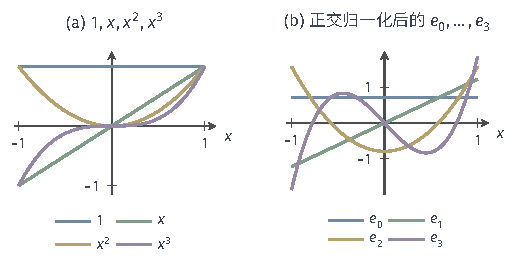
\includegraphics[width=87.3mm]{figures/02-abstract-mathematics/03-function-spaces/tikz/c1-legendre-gram-schmidt/figure.pdf}
  \caption{在$L^2[-1,1]$中对单项式做Gram--Schmidt正交化。(a)$1,x,x^2,x^3$，例如$\langle1,x^2\rangle=\tfrac23\neq0$；(b)得到的$e_0=1/\sqrt2$，$e_1=\sqrt{3/2}\,x$，$e_2=\sqrt{5/8}\,(3x^2-1)$，$e_3=\sqrt{7/8}\,(5x^3-3x)$，两两正交且范数为$1$，$e_k$在$(-1,1)$内恰有$k$个零点。}
  \label{fig:ipspace-legendre-gram-schmidt}
\end{figure}

\paragraph{完备正交系}
一个标准正交系“够不够用”，看它的有限组合能否逼近每个元素。$\{e_i\}$的有限线性组合全体记为$\operatorname{span}\{e_i\}$，它在$H$中的闭包记为$\overline{\operatorname{span}}\{e_i\}$，称为\term{闭线性张成}（closed linear span）。

\begin{definition}[完备正交系]
\label{def:ipspace-complete-orthonormal-system}
若Hilbert空间$H$中的标准正交系$\{e_i\}_{i\in I}$满足$\overline{\operatorname{span}}\{e_i\}=H$，称它为$H$的\term{完备正交系}（complete orthonormal system），也称\term{标准正交基}（orthonormal basis）或正交基。
\end{definition}

这里的“完备”与空间的完备是两个不同的概念：前者说正交系的方向够用，后者说柯西列有极限。“基”字也要小心理解。代数基要求每个元素恰是有限个基元素的组合；正交基只要求每个元素是有限组合的范数极限，允许通过极限逼近。下一节将说明，这样的极限可以写成按范数收敛的级数。

$\ell^2$中的标准单位列是完备正交系。对$x\in\ell^2$，截断$x^{(N)}=\sum_{k\leq N}x_ke_k\in\operatorname{span}\{e_k\}$满足
\[
 \lVert x-x^{(N)}\rVert^2=\sum_{k>N}\lvert x_k\rvert^2\to0,
\]
因为收敛级数的尾和趋于零。所以$\operatorname{span}\{e_k\}=c_{00}$在$\ell^2$中稠密。但$\{e_k\}$不是$\ell^2$的代数基：$(1,\tfrac12,\tfrac13,\ldots)\in\ell^2$有无穷多项非零，不是有限个$e_k$的组合。

\paragraph{完备性的正交判据}
判断一个标准正交系是否完备，常用的办法是看还有没有被它遗漏的方向。

\begin{theorem}[完备正交系的判据]
\label{thm:ipspace-completeness-criterion}
设$\{e_i\}_{i\in I}$是Hilbert空间$H$中的标准正交系。则它是完备正交系，当且仅当与每个$e_i$都正交的元素只有零。
\end{theorem}

\begin{proof}
记$M=\overline{\operatorname{span}}\{e_i\}$，它是闭线性子空间。设$M=H$，$g$与每个$e_i$正交。由内积的线性，$g$与$\operatorname{span}\{e_i\}$正交；由内积的连续性，$g$也与其闭包$M=H$正交，特别地$\langle g,g\rangle=0$，$g=0$。

反过来，设$M\neq H$，取$f\notin M$。由第~\ref{sec:ipspace-orthogonal-projection}节，$g=f-P_Mf$属于$M^\perp$，且$g\neq0$，因为$P_Mf\in M$而$f\notin M$。这个$g$与每个$e_i$正交，所以判据的条件不成立。
\end{proof}

判据的“必要”方向只用到内积的连续性，“充分”方向用到了正交投影，从而用到了完备性与闭性。例如在$L^2[-1,1]$中，偶次的归一化Legendre多项式$e_0,e_2,e_4,\ldots$组成一个无穷的标准正交系，但$x$是奇函数，与每个偶函数正交，而$x\neq0$。所以这个系不完备：方向有无穷多个，却遗漏了全部奇函数。

全体Legendre多项式$\{e_k\}_{k\geq0}$是否完备，取决于多项式能否在$L^2[-1,1]$中逼近每个元素。这需要两步逼近：连续函数在$L^2[-1,1]$中稠密，多项式又能一致逼近连续函数。这两步属于第~\ref{chap:function-approximation}章，这里不给出证明，只指出结论：Legendre多项式是$L^2[-1,1]$的完备正交系。

\paragraph{可分空间的可数正交基}
要用级数$\sum_jc_je_j$表示每个元素，正交基最好是可数的。第~\ref{chap:topological-spaces}章把具有可数稠密子集的空间称为\term{可分}（separable）空间。下面说明，对Hilbert空间而言，“有可数的正交基”与“可分”是一回事。

\begin{theorem}[可分Hilbert空间的正交基]
\label{thm:ipspace-separable-basis}
设$H$是可分Hilbert空间，$H\neq\{0\}$。则$H$有至多可数的标准正交基，并且$H$中每个标准正交系都至多可数。
\end{theorem}

\begin{proof}
取可数稠密子集$\{u_k\}_{k\geq1}$。依次检查各项，删去能由前面保留的项线性表示的项，得到一个线性无关的序列（有限或无限），其张成空间与$\operatorname{span}\{u_k\}$相同。对它做Gram--Schmidt正交化，得到标准正交系$\{e_j\}$，其张成空间仍与$\operatorname{span}\{u_k\}$相同。这个张成空间包含稠密集$\{u_k\}$，所以在$H$中稠密，$\{e_j\}$是至多可数的完备正交系。

再设$\{e_i\}_{i\in I}$是任意标准正交系。对$i\neq j$，$\lVert e_i-e_j\rVert^2=\lVert e_i\rVert^2+\lVert e_j\rVert^2=2$。所以以各$e_i$为中心、半径$\tfrac{\sqrt2}2$的开球两两不交。每个开球都含有稠密集$\{u_k\}$中的点，不同的球含有不同的点，于是$i\mapsto$（球中某个$u_k$的下标$k$）是$I$到$\mathbb N_+$的单射，$I$至多可数。
\end{proof}

反方向也成立：若$H$有可数的正交基$\{e_j\}$，则系数取有理数（复情形取实部、虚部为有理数）的有限组合构成可数集，并且在$H$中稠密，所以$H$可分。$\ell^2$有可数的正交基$\{e_k\}$，因而可分；由上面所述的Legendre多项式的完备性，$L^2[-1,1]$也可分。不可分的Hilbert空间也存在，那时正交基不可数，下一节的级数需要改写为不可数族的求和，本书不展开。
